% Created by tikzDevice version 0.10.1 on 2018-02-09 14:43:10
% !TEX encoding = UTF-8 Unicode
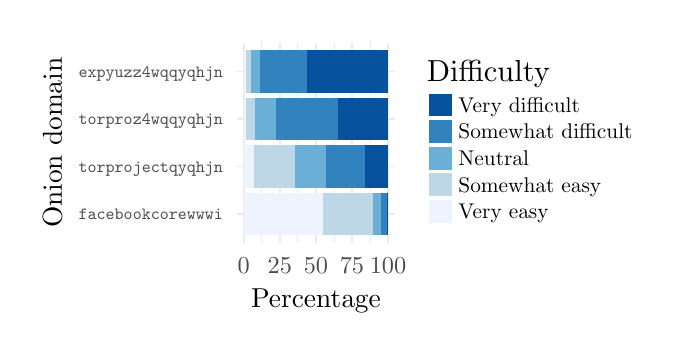
\begin{tikzpicture}[x=1pt,y=1pt]
\definecolor{fillColor}{RGB}{255,255,255}
\path[use as bounding box,fill=fillColor,fill opacity=0.00] (0,0) rectangle (224.04,108.41);
\begin{scope}
\path[clip] ( 75.47, 30.77) rectangle (132.84,102.91);
\definecolor{drawColor}{gray}{0.92}

\path[draw=drawColor,line width= 0.3pt,line join=round] ( 84.60, 30.77) --
	( 84.60,102.91);

\path[draw=drawColor,line width= 0.3pt,line join=round] ( 97.64, 30.77) --
	( 97.64,102.91);

\path[draw=drawColor,line width= 0.3pt,line join=round] (110.67, 30.77) --
	(110.67,102.91);

\path[draw=drawColor,line width= 0.3pt,line join=round] (123.71, 30.77) --
	(123.71,102.91);

\path[draw=drawColor,line width= 0.6pt,line join=round] ( 75.47, 41.08) --
	(132.84, 41.08);

\path[draw=drawColor,line width= 0.6pt,line join=round] ( 75.47, 58.25) --
	(132.84, 58.25);

\path[draw=drawColor,line width= 0.6pt,line join=round] ( 75.47, 75.43) --
	(132.84, 75.43);

\path[draw=drawColor,line width= 0.6pt,line join=round] ( 75.47, 92.60) --
	(132.84, 92.60);

\path[draw=drawColor,line width= 0.6pt,line join=round] ( 78.08, 30.77) --
	( 78.08,102.91);

\path[draw=drawColor,line width= 0.6pt,line join=round] ( 91.12, 30.77) --
	( 91.12,102.91);

\path[draw=drawColor,line width= 0.6pt,line join=round] (104.16, 30.77) --
	(104.16,102.91);

\path[draw=drawColor,line width= 0.6pt,line join=round] (117.19, 30.77) --
	(117.19,102.91);

\path[draw=drawColor,line width= 0.6pt,line join=round] (130.23, 30.77) --
	(130.23,102.91);
\definecolor{fillColor}{RGB}{239,243,255}

\path[fill=fillColor] ( 78.08, 33.35) rectangle (106.78, 48.81);
\definecolor{fillColor}{RGB}{189,215,231}

\path[fill=fillColor] (106.78, 33.35) rectangle (124.77, 48.81);
\definecolor{fillColor}{RGB}{107,174,214}

\path[fill=fillColor] (124.77, 33.35) rectangle (127.56, 48.81);
\definecolor{fillColor}{RGB}{49,130,189}

\path[fill=fillColor] (127.56, 33.35) rectangle (129.70, 48.81);
\definecolor{fillColor}{RGB}{8,81,156}

\path[fill=fillColor] (129.70, 33.35) rectangle (130.24, 48.81);
\definecolor{fillColor}{RGB}{239,243,255}

\path[fill=fillColor] ( 78.08, 50.52) rectangle ( 81.93, 65.98);
\definecolor{fillColor}{RGB}{189,215,231}

\path[fill=fillColor] ( 81.93, 50.52) rectangle ( 96.50, 65.98);
\definecolor{fillColor}{RGB}{107,174,214}

\path[fill=fillColor] ( 96.50, 50.52) rectangle (107.64, 65.98);
\definecolor{fillColor}{RGB}{49,130,189}

\path[fill=fillColor] (107.64, 50.52) rectangle (121.88, 65.98);
\definecolor{fillColor}{RGB}{8,81,156}

\path[fill=fillColor] (121.88, 50.52) rectangle (130.24, 65.98);
\definecolor{fillColor}{RGB}{239,243,255}

\path[fill=fillColor] ( 78.08, 67.70) rectangle ( 78.94, 83.15);
\definecolor{fillColor}{RGB}{189,215,231}

\path[fill=fillColor] ( 78.94, 67.70) rectangle ( 82.05, 83.15);
\definecolor{fillColor}{RGB}{107,174,214}

\path[fill=fillColor] ( 82.05, 67.70) rectangle ( 89.67, 83.15);
\definecolor{fillColor}{RGB}{49,130,189}

\path[fill=fillColor] ( 89.67, 67.70) rectangle (112.21, 83.15);
\definecolor{fillColor}{RGB}{8,81,156}

\path[fill=fillColor] (112.21, 67.70) rectangle (130.24, 83.15);
\definecolor{fillColor}{RGB}{239,243,255}

\path[fill=fillColor] ( 78.08, 84.87) rectangle ( 78.73,100.33);
\definecolor{fillColor}{RGB}{189,215,231}

\path[fill=fillColor] ( 78.73, 84.87) rectangle ( 80.78,100.33);
\definecolor{fillColor}{RGB}{107,174,214}

\path[fill=fillColor] ( 80.78, 84.87) rectangle ( 83.80,100.33);
\definecolor{fillColor}{RGB}{49,130,189}

\path[fill=fillColor] ( 83.80, 84.87) rectangle (100.82,100.33);
\definecolor{fillColor}{RGB}{8,81,156}

\path[fill=fillColor] (100.82, 84.87) rectangle (130.23,100.33);
\end{scope}
\begin{scope}
\path[clip] (  0.00,  0.00) rectangle (224.04,108.41);
\definecolor{drawColor}{gray}{0.30}

\node[text=drawColor,anchor=base east,inner sep=0pt, outer sep=0pt, scale=  0.62] at ( 70.52, 38.96) {\texttt{facebookcorewwwi}};

\node[text=drawColor,anchor=base east,inner sep=0pt, outer sep=0pt, scale=  0.62] at ( 70.52, 56.13) {\texttt{torprojectqyqhjn}};

\node[text=drawColor,anchor=base east,inner sep=0pt, outer sep=0pt, scale=  0.62] at ( 70.52, 73.30) {\texttt{torproz4wqqyqhjn}};

\node[text=drawColor,anchor=base east,inner sep=0pt, outer sep=0pt, scale=  0.62] at ( 70.52, 90.48) {\texttt{expyuzz4wqqyqhjn}};
\end{scope}
\begin{scope}
\path[clip] (  0.00,  0.00) rectangle (224.04,108.41);
\definecolor{drawColor}{gray}{0.30}

\node[text=drawColor,anchor=base,inner sep=0pt, outer sep=0pt, scale=  0.88] at ( 78.08, 19.76) {0};

\node[text=drawColor,anchor=base,inner sep=0pt, outer sep=0pt, scale=  0.88] at ( 91.12, 19.76) {25};

\node[text=drawColor,anchor=base,inner sep=0pt, outer sep=0pt, scale=  0.88] at (104.16, 19.76) {50};

\node[text=drawColor,anchor=base,inner sep=0pt, outer sep=0pt, scale=  0.88] at (117.19, 19.76) {75};

\node[text=drawColor,anchor=base,inner sep=0pt, outer sep=0pt, scale=  0.88] at (130.23, 19.76) {100};
\end{scope}
\begin{scope}
\path[clip] (  0.00,  0.00) rectangle (224.04,108.41);
\definecolor{drawColor}{RGB}{0,0,0}

\node[text=drawColor,anchor=base,inner sep=0pt, outer sep=0pt, scale=  0.99] at (104.16,  7.44) {Percentage};
\end{scope}
\begin{scope}
\path[clip] (  0.00,  0.00) rectangle (224.04,108.41);
\definecolor{drawColor}{RGB}{0,0,0}

\node[text=drawColor,rotate= 90.00,anchor=base,inner sep=0pt, outer sep=0pt, scale=  0.99] at ( 12.32, 66.84) {Onion domain};
\end{scope}
\begin{scope}
\path[clip] (  0.00,  0.00) rectangle (224.04,108.41);
\definecolor{drawColor}{RGB}{0,0,0}

\node[text=drawColor,anchor=base west,inner sep=0pt, outer sep=0pt, scale=  1.10] at (144.23, 88.95) {Difficulty};
\end{scope}
\begin{scope}
\path[clip] (  0.00,  0.00) rectangle (224.04,108.41);
\definecolor{fillColor}{RGB}{8,81,156}

\path[fill=fillColor] (144.94, 76.41) rectangle (153.15, 84.62);
\end{scope}
\begin{scope}
\path[clip] (  0.00,  0.00) rectangle (224.04,108.41);
\definecolor{fillColor}{RGB}{49,130,189}

\path[fill=fillColor] (144.94, 66.77) rectangle (153.15, 74.99);
\end{scope}
\begin{scope}
\path[clip] (  0.00,  0.00) rectangle (224.04,108.41);
\definecolor{fillColor}{RGB}{107,174,214}

\path[fill=fillColor] (144.94, 57.14) rectangle (153.15, 65.35);
\end{scope}
\begin{scope}
\path[clip] (  0.00,  0.00) rectangle (224.04,108.41);
\definecolor{fillColor}{RGB}{189,215,231}

\path[fill=fillColor] (144.94, 47.50) rectangle (153.15, 55.72);
\end{scope}
\begin{scope}
\path[clip] (  0.00,  0.00) rectangle (224.04,108.41);
\definecolor{fillColor}{RGB}{239,243,255}

\path[fill=fillColor] (144.94, 37.87) rectangle (153.15, 46.08);
\end{scope}
\begin{scope}
\path[clip] (  0.00,  0.00) rectangle (224.04,108.41);
\definecolor{drawColor}{RGB}{0,0,0}

\node[text=drawColor,anchor=base west,inner sep=0pt, outer sep=0pt, scale=  0.77] at (155.67, 77.86) {Very difficult};
\end{scope}
\begin{scope}
\path[clip] (  0.00,  0.00) rectangle (224.04,108.41);
\definecolor{drawColor}{RGB}{0,0,0}

\node[text=drawColor,anchor=base west,inner sep=0pt, outer sep=0pt, scale=  0.77] at (155.67, 68.23) {Somewhat difficult};
\end{scope}
\begin{scope}
\path[clip] (  0.00,  0.00) rectangle (224.04,108.41);
\definecolor{drawColor}{RGB}{0,0,0}

\node[text=drawColor,anchor=base west,inner sep=0pt, outer sep=0pt, scale=  0.77] at (155.67, 58.59) {Neutral};
\end{scope}
\begin{scope}
\path[clip] (  0.00,  0.00) rectangle (224.04,108.41);
\definecolor{drawColor}{RGB}{0,0,0}

\node[text=drawColor,anchor=base west,inner sep=0pt, outer sep=0pt, scale=  0.77] at (155.67, 48.96) {Somewhat easy};
\end{scope}
\begin{scope}
\path[clip] (  0.00,  0.00) rectangle (224.04,108.41);
\definecolor{drawColor}{RGB}{0,0,0}

\node[text=drawColor,anchor=base west,inner sep=0pt, outer sep=0pt, scale=  0.77] at (155.67, 39.32) {Very easy};
\end{scope}
\end{tikzpicture}
